\begin{frame}{Robot Scara 4 bậc tự do}
    \begin{columns}
        \column{0.5\textwidth}
        \begin{itemize}
            \item Robot Scara có 4 bậc tự do biểu diễn qua các tọa độ: \( q = [q_1, q_2, q_3, q_4]^T \).
            \item 3 khớp quay: \(q_1\), \(q_2\), \(q_4\).
            \item 1 khớp tịnh tiến: \(q_3\).
        \end{itemize}
        \begin{figure}
            \centering
            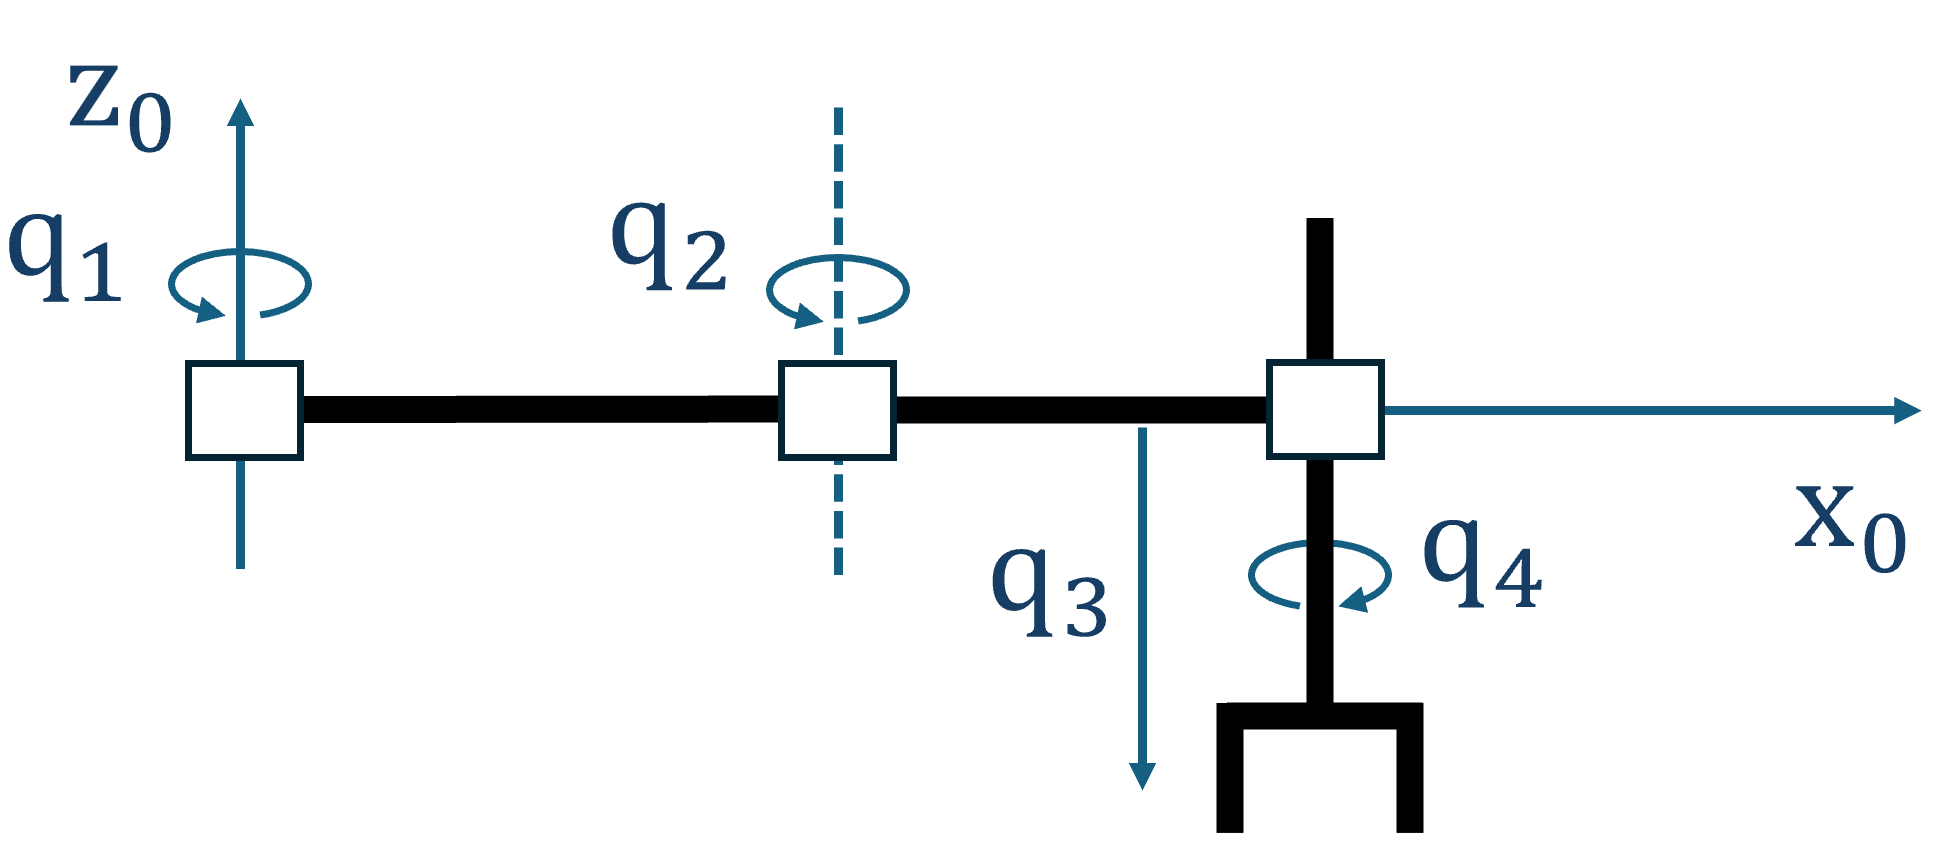
\includegraphics[width=0.8\linewidth]{Figures/Scara_xOz.png}
            \caption{Mặt cắt phương xOz của Robot Scara.}
            \label{fig:Scara_xOz}
        \end{figure}
        \column{0.5\textwidth}
        \begin{figure}
            \centering
            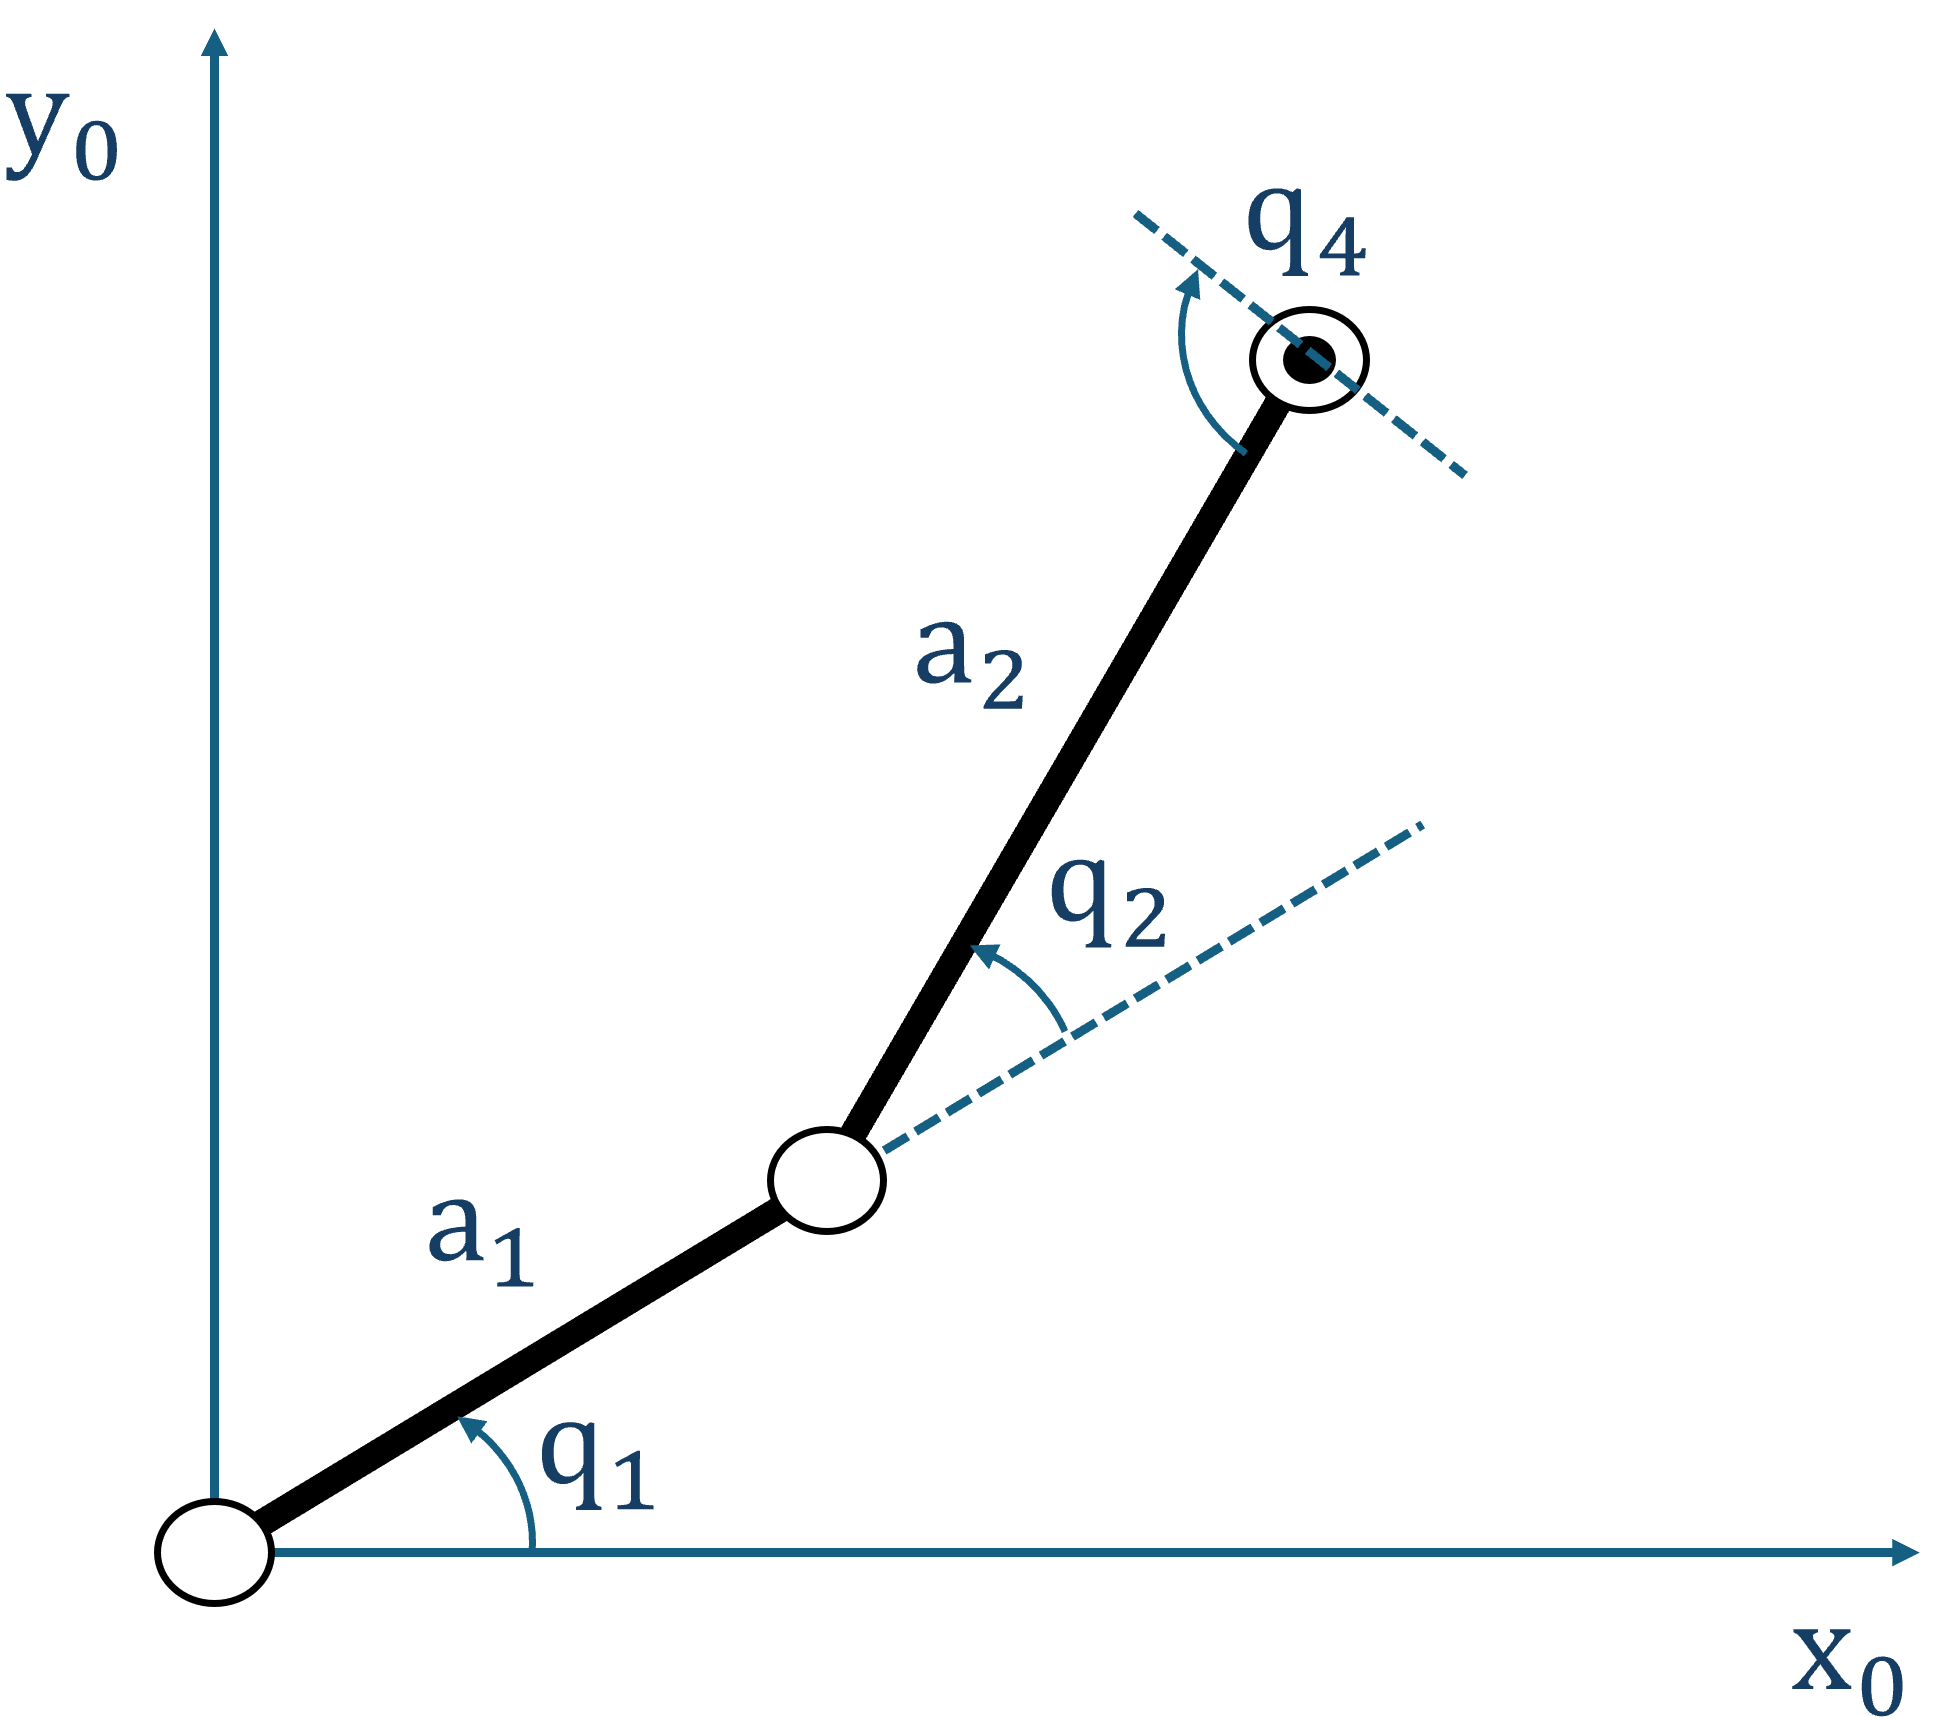
\includegraphics[width=0.8\linewidth]{Figures/Scara_xOy.png}
            \caption{Mặt cắt phương xOy của Robot Scara.}
            \label{fig:Scara_xOy}
        \end{figure}
    \end{columns}
\end{frame}